\chapter{Continous Integration}


Have you ever had a situation when your software has a bug but it is
not discovered for a long time?  The existence of the bug and its
ability to escape detection may surprise your entire team. ``How did
that happen?'', you may ask.  This may happen due to a wide variety of
reasons. One of the possible reasons is that the software has not been
well tested and as a result the bug is not detected. Testing is an
important method detecting bugs.  However, testing can be tideous.  It
is common that someone makes a ``small'' change and skips testing.
The person believes the change is so small and cannot possibly have
any bug.  If several people add a few small changes here and there,
the software soon is full of ``small'' bugs.  Why do people not test
their programs immediately after they have made changes?  One reason
is that testing require additional work.

Is it possible testing is fully automated without any additional
effort? {\it Continuous Integration} (CI) does exactly that.

You still need to write testers. There is no way avoiding that part.
What continuous integration does is to automatically invole these
testers whenver you push your program to the shared repository.
This chapter uses {\tt Travis-CI} for continuous integration.

\begin{figure}[h] \centering
{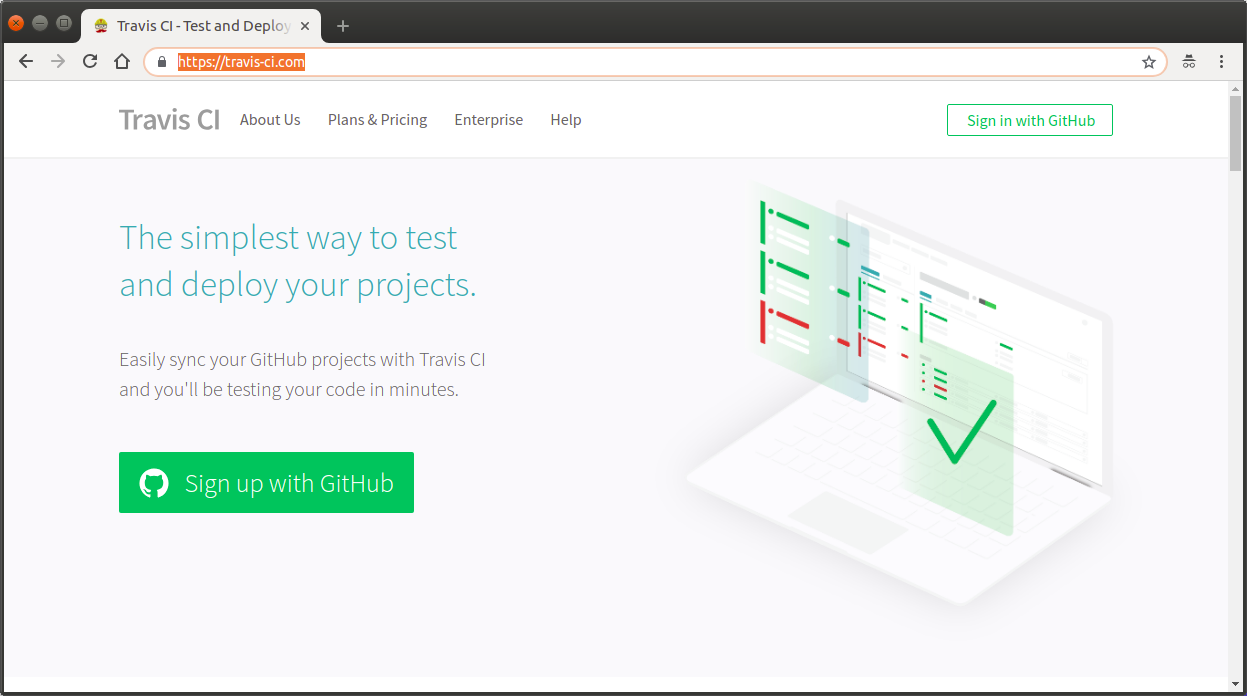
\includegraphics[width=4.5in]{\thischapterpath/figures/travis01.png}}
\caption{Travis-CI.com is a website supporting continuous integration.}
\label{fig:travis01}
\end{figure}
